
\documentclass[a4paper,11pt]{article}%,twocolumn
%% packages

\usepackage{blindtext} % needed for creating dummy text passages
%\usepackage{ngerman} % needed for German default language
\usepackage{amsmath} % needed for command eqref
\usepackage{amssymb} % needed for math fonts
\usepackage[colorlinks=true,breaklinks]{hyperref} % needed for creating hyperlinks in the document, the option colorlinks=true gets rid of the awful boxes, breaklinks breaks lonkg links (list of figures), and ngerman sets everything for german as default hyperlinks language
\usepackage[hyphenbreaks]{breakurl} % ben�tigt f�r das Brechen von URLs in Literaturreferenzen, hyphenbreaks auch bei links, die �ber eine Seite gehen (mit hyphenation).
\usepackage{xcolor}
\definecolor{c1}{rgb}{0,0,1} % blue
\definecolor{c2}{rgb}{0,0.3,0.9} % light blue
\definecolor{c3}{rgb}{0.3,0,0.9} % red blue
\hypersetup{
    linkcolor={c1}, % internal links
    citecolor={c2}, % citations
    urlcolor={c3} % external links/urls
}
%\usepackage{cite} % needed for cite
\usepackage[square,authoryear]{natbib} % needed for cite and abbrvnat bibliography style
\usepackage[nottoc]{tocbibind} % needed for displaying bibliography and other in the table of contents
\usepackage{graphicx} % needed for \includegraphics 
\usepackage{longtable} % needed for long tables over pages
\usepackage{bigstrut} % needed for the command \bigstrut
\usepackage{enumerate} % needed for some options in enumerate
%\usepackage{todonotes} % needed for todos
\usepackage{makeidx} % needed for creating an index
\makeindex
\usepackage{gensymb}
\usepackage{url}
\usepackage{psfrag}
\usepackage{multirow}
\usepackage{subfigure}
%% page settings

\usepackage[top=20mm, bottom=20mm,left=15mm,right=15mm]{geometry} % needed for page border settings
\parindent=0mm % for space of first line of new text block
\sloppy % for writing with hyphenless justification (tries to)
\hyphenation{} % use hyphenation of tolerance parametershttp://www.jr-x.de/publikationen/latex/tipps/zeilenumbruch.html
\hyphenpenalty=10000
\exhyphenpenalty=10000
\usepackage{fancyhdr} % needed for head and foot options
%% my macros

%% Text fomats
\newcommand{\tbi}[1]{\textbf{\textit{#1}}}

%% Math fonts
\newcommand{\bbA}{\mathbb{A}}
\newcommand{\bbB}{\mathbb{B}}
\newcommand{\bbC}{\mathbb{C}}
\newcommand{\bbD}{\mathbb{D}}
\newcommand{\bbE}{\mathbb{E}}
\newcommand{\bbF}{\mathbb{F}}
\newcommand{\bbG}{\mathbb{G}}
\newcommand{\bbH}{\mathbb{H}}
\newcommand{\bbI}{\mathbb{I}}
\newcommand{\bbJ}{\mathbb{J}}
\newcommand{\bbK}{\mathbb{K}}
\newcommand{\bbL}{\mathbb{L}}
\newcommand{\bbM}{\mathbb{M}}
\newcommand{\bbN}{\mathbb{N}}
\newcommand{\bbO}{\mathbb{O}}
\newcommand{\bbP}{\mathbb{P}}
\newcommand{\bbQ}{\mathbb{Q}}
\newcommand{\bbR}{\mathbb{R}}
\newcommand{\bbS}{\mathbb{S}}
\newcommand{\bbT}{\mathbb{T}}
\newcommand{\bbU}{\mathbb{U}}
\newcommand{\bbV}{\mathbb{V}}
\newcommand{\bbW}{\mathbb{W}}
\newcommand{\bbX}{\mathbb{X}}
\newcommand{\bbY}{\mathbb{Y}}
\newcommand{\bbZ}{\mathbb{Z}}
\usepackage[ framed, numbered]{matlab-prettifier}%framed,%
\usepackage{listings}
\usepackage{physics}
\usepackage{pdfpages}
\usepackage[toc,page]{appendix}
\usepackage{float}
\usepackage{hyperref}

\newenvironment{qanda}{\setlength{\parindent}{0pt}}{\bigskip}
\newcommand{\Q}{\bigskip\bfseries Q: }
\newcommand{\A}{\par\textbf{Answer: } \normalfont}

\begin{document}
\begin{titlepage}
\center % Center everything on the page

%-------------------------------------------------------------------------------------
%	HEADING SECTIONS
%------------------------------------------------------------------------------------
\textbf{\large Department of Electrical and Computer Engineering}\\[0.5cm]
\textbf{\Large University of Colorado at Boulder}\\[1cm]
\textbf{\large ECEN5623 - Real Time Embedded Systems }\\[2cm]

\includegraphics[width=0.3\textwidth]{figures/cu}\\[2cm]

	
%-------------------------------------------------------------------------------------
%	TITLE SECTION
%------------------------------------------------------------------------------------
\textbf{\Huge Exercise 5 }\\[0.2cm]



%----------------------------------------------------------------------------------------
%	MEMBERS SECTION
%----------------------------------------------------------------------------------------


\vfill

\textbf{\large Submitted by}\\[0.5cm]

{\large Parth | Jithedra}\\[0.5cm]	

%----------------------------------------------------------------------------------------
%	DATE SECTION
%----------------------------------------------------------------------------------------

\textbf{\large Submitted on}
\textbf{\Large \today} % Date, change the \today to a set date if you want to be precise

%----------------------------------------------------------------------------------------

\vfill % Fill the rest of the page with whitespace

\end{titlepage}


\pagebreak

\tableofcontents
\listoffigures
\listoftables
\vfill
\begin{center}
	\textbf{\textit{*PDF is clickable}}
\end{center}

\pagebreak



\begin{qanda}

	\section{Question 1}
	\Q  Create a user-defined interrupt handler for the timer ISR and a task for processing. The timer should
	be scheduled on a regular basis, and the interrupt handler should signal the processing task. To ensure
	that the timer is being triggered with the correct periodicity, pass the interrupt timing to the processing
	task.
	\addcontentsline{toc}{subsection}{Answer}
	\A

	Code Flow and Meaning:
	\begin{enumerate}
		\item The code starts by including the necessary header files:
		\begin{itemize}
			\item <stdint.h> and <stdbool.h> for standard integer types and boolean type.
			\item "main.h" and "drivers/pinout.h" for project-specific configurations and pin definitions.
			\item "utils/uartstdio.h" for UART communication functionality.
			Various TivaWare header files ("driverlib/...") for accessing TivaC hardware features.
			\item Various TivaWare header files ("driverlib/...") for accessing TivaC hardware features.
			\item FreeRTOS header files ("FreeRTOS.h", "task.h", "queue.h", etc.) for using FreeRTOS functionality.
		\end{itemize}
		\item The code declares global variables:
		\begin{itemize}
			\item task1SyncSemaphore is a binary semaphore handle used for synchronization.
			\item Task1\_handle is a task handle for xTask1.
			\item Hz is set to 100, representing the desired frequency for the timer interrupt.
			\item ulPeriod is used to store the calculated timer period.
		\end{itemize}
		\item The Timer0Isr() function is the timer interrupt service routine (ISR)
		\begin{itemize}
			\item It is called whenever the Timer0 interrupt occurs.
			\item It retrieves the current tick count using xTaskGetTickCount().
			\item It clears the timer interrupt flag using ROM\_TimerIntClear().
			\item It sends a task notification to Task1\_handle using xTaskNotifyFromISR(), passing the current tick count as the notification value.
		\end{itemize}
		\item The xTask1() function is the task that waits for the timer notification:
		\begin{itemize}
			\item It is created with a stack size of configMINIMAL\_STACK\_SIZE and a priority of 2.
			\item It enters an infinite loop.
			\item Inside the loop, it waits for a notification using xTaskNotifyWait() with a maximum block time of 5000 ms.
			\item If a notification is received (xResult == pdPASS), it retrieves the current tick count and the notified value.
			\item It prints a message using UARTprintf(), indicating the task completion time and the received timer interrupt data (tick count).
		\end{itemize}
		\item The main() function is the entry point of the program:
		\begin{itemize}
			\item It initializes the system clock to 120 MHz using ROM\_SysCtlClockFreqSet().
			\item It initializes the GPIO pins for the LaunchPad using PinoutSet().
			\item It configures the UART for stdio output at a baud rate of 230400 using UARTStdioConfig().
			\item It enables and configures Timer0 as a periodic timer using ROM\_SysCtlPeripheralEnable() and ROM\_TimerConfigure().
			\item It registers the timer ISR Timer0Isr() using TimerIntRegister().
			\item It calculates the timer period based on the desired frequency (Hz) and the system clock rate.
			\item It loads the timer with the calculated period using ROM\_TimerLoadSet() and enables the timer using ROM\_TimerEnable().
			\item It enables the Timer0 interrupt using ROM\_IntEnable() and ROM\_TimerIntEnable().
			\item It creates a binary semaphore task1SyncSemaphore using xSemaphoreCreateBinary().
			\item It creates the task xTask1 using xTaskCreate().
			\item Finally, it starts the FreeRTOS scheduler using vTaskStartScheduler().
		\end{itemize}
	\end{enumerate}
	
	\begin{figure}[!h]
		\centering
		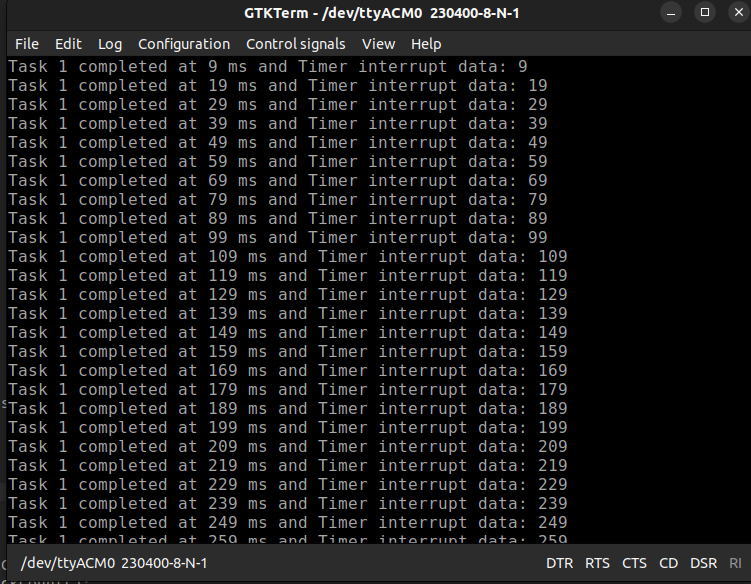
\includegraphics[scale=0.6]{figures/q1.png}
		\caption{Semaphore has been posted by this program}

	\end{figure}


	Output Analysis:
	\begin{enumerate}
		\item The output of the code, as shown in the provided screenshot, displays the task completion messages printed by xTask1 at regular intervals. Each message includes the task completion time in milliseconds and the timer interrupt data (tick count) received through the notification.
		
	\end{enumerate}
	
	
	Here's a detailed analysis of the output:
	\begin{enumerate}
		\item The first message indicates that Task 1 completed at 9 ms, and the timer interrupt data received is 9. This means that the first timer interrupt occurred at around 9 ms after the program started, and xTask1 received the notification with the tick count value of 9.
		\item The subsequent messages show that Task 1 completes at regular intervals of approximately 10 ms, which corresponds to the timer frequency of 100 Hz. For example, the second message shows Task 1 completing at 19 ms with a timer interrupt data of 19, indicating that the second timer interrupt occurred 10 ms after the first one.
		\item The tick count value in each message increments by 10 ms compared to the previous message. This confirms that the timer interrupt is occurring at the specified frequency of 100 Hz, and the tick count is accurately reflecting the time elapsed since the program started.
		\item The output continues with Task 1 completing at 29 ms, 39 ms, 49 ms, and so on, with the corresponding timer interrupt data matching the completion time. This demonstrates the consistent and accurate synchronization between the timer interrupt and the task notification.
		The program keeps running indefinitely, with xTask1 receiving notifications and printing messages at regular intervals of 10 ms, until it is manually stopped or the desired runtime is reached.
	\end{enumerate}
	
	
	
	
	
	The output verifies that the code is functioning as intended, with the timer interrupt triggering at the specified frequency of 100 Hz and xTask1 receiving notifications and printing the task completion time and timer interrupt data accordingly. This confirms the successful setup and synchronization between the timer interrupt and the task using FreeRTOS task notifications.
	
	
	
	\pagebreak
	\section{Question 2}
	\Q   Create a pair of FreeRTOS tasks that signal each other. The first task performs some computation,
	signals the other task, and waits for a signal from that task. The second task repeats the same pattern
	so that they alternate. Each task should complete a defined amount of work, such as computing a
	specified number of Fibonacci values or some equivalent synthetic load. Do not use sleep functions as a
	load. Profile each task, by storing timestamps that can be printed at the end, with one task executing
	for 10 ms and the other for 40 ms. Run for at least 200 ms. Printing can be done using UARTprintf().
	\addcontentsline{toc}{subsection}{Answer}
	\A

	The goal of this question is to create two FreeRTOS tasks that communicate with each other using signals (semaphores) and perform computations alternately. The tasks should follow a specific pattern of execution:
\begin{enumerate}
	\item Task 1 performs a computation, signals Task 2, and then waits for a signal from Task 2.
	\item Task 2, upon receiving the signal from Task 1, performs its computation, signals Task 1, and waits for a signal from Task 1.
	\item This pattern repeats, with the tasks alternating their execution.
\end{enumerate}


Each task should have a defined amount of work to complete, such as calculating a specific number of Fibonacci values or any other computational load. It's important to note that sleep functions should not be used as a load, as they would not represent actual computational work.\\

Profiling is required to measure the execution time of each task. Timestamps should be stored at appropriate points in the code to track the start and end times of each task's execution. The goal is to have Task 1 execute for approximately 10 milliseconds and Task 2 execute for approximately 40 milliseconds in each iteration.\\

The overall program should run for at least 200 milliseconds to allow for multiple iterations of the alternating task execution.\\

Finally, the stored timestamps and any relevant information should be printed using the UARTprintf() function, which sends the output to the UART (Universal Asynchronous Receiver/Transmitter) for display or logging purposes.\\

Detailed Code Analysis:
\begin{enumerate}
	\item The fiboncacci() function is defined to calculate Fibonacci numbers for a specified duration in milliseconds. It uses a loop to calculate Fibonacci numbers up to FIB\_LIMIT\_FOR\_32\_BIT and keeps track of the elapsed time using xTaskGetTickCount().
	\item The xTask1() function represents the first task:
	\begin{itemize}
		\item It enters a loop that runs until the total runtime (TIME\_TO\_RUN) is reached.
		\item Inside the loop, it waits for the task1SyncSemaphore using xSemaphoreTake().
		\item Once the semaphore is obtained, it calls the fiboncacci() function to perform calculations for 10 ms.
		\item After the calculations, it prints the current time and the time taken to execute the Fibonacci function using UARTprintf().
		\item Finally, it gives the task2SyncSemaphore to signal Task 2.
		The xTask2() function represents the second task and follows a similar 
	\end{itemize}
	\item pattern as xTask1():
	\begin{itemize}
		\item It waits for the task2SyncSemaphore.
		\item Upon receiving the semaphore, it performs Fibonacci calculations for 40 ms.
		\item It prints the execution time using UARTprintf().
		\item It gives the task1SyncSemaphore to signal Task 1.
	\end{itemize}
	
	\item The main() function serves as the entry point of the program:
	\begin{itemize}
		\item It initializes the system clock, GPIO pins, and UART using the provided TivaWare functions.
		\item It creates the semaphores task1SyncSemaphore and task2SyncSemaphore using xSemaphoreCreateBinary().
		\item It creates xTask1 and xTask2 using xTaskCreate(), specifying their respective function names, stack sizes, and priorities.
		\item The task1SyncSemaphore is given initially to start the alternating execution.
		\item The startTimeTick is recorded to keep track of the total runtime.
		\item 
		Finally, the FreeRTOS scheduler is started using vTaskStartScheduler().
		
	\end{itemize}
	
	
\end{enumerate}




\begin{figure}[!h]
	\centering
	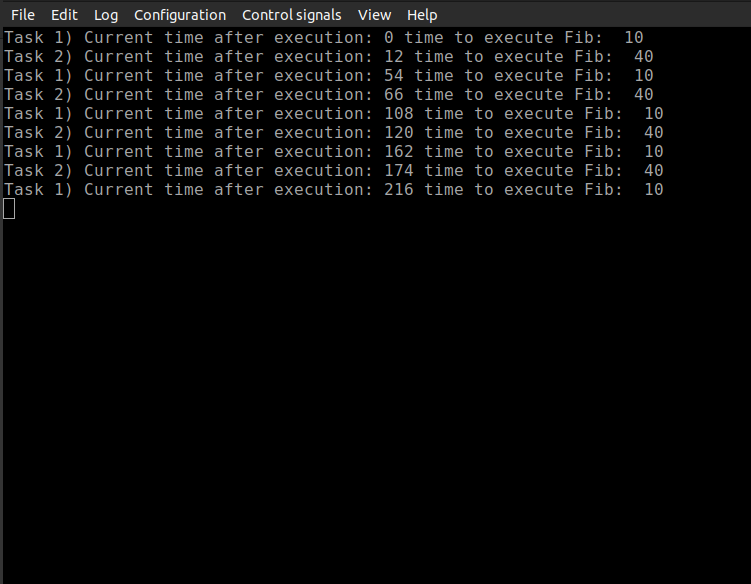
\includegraphics[scale=0.6]{figures/q2.png}
	\caption{Semaphore has been posted by this program}

\end{figure}

Detailed Output Analysis:

The provided screenshot shows the output of the program, which demonstrates the alternating execution of Task 1 and Task 2 and their respective execution times.
\begin{enumerate}
	\item The first line of the output indicates that Task 1 executed at time 0 and took 10 ms to execute the Fibonacci calculations. This is the initial execution of Task 1.
	\item The second line shows that Task 2 executed again at time 12 and took 40 ms for the Fibonacci calculations. This implies that Task 2 executed between the first and second executions of Task 1, taking approximately 2 ms (12 - 10 = 2 ms) for its own execution and signaling.
	\item 
\end{enumerate}


The subsequent lines follow the alternating pattern of Task 1 and Task 2 execution:
Task 1 executes at time 54, taking 10 ms for Fibonacci calculations.
Task 2 executes again at time 66, indicating that Task 2 executed in between and took approximately 2 ms (66 - 54 - 10 = 2 ms).
This pattern continues, with Task 1 executing for 10 ms and Task 2 executing for 40 ms in each iteration.
The output continues until the total runtime of 200 ms is reached, as specified by the TIME\_TO\_RUN constant.
The output demonstrates the successful synchronization and alternating execution of Task 1 and Task 2 using semaphores. The timestamps printed show the precise execution times of each task and the time taken for the Fibonacci calculations.\\

The analysis reveals that Task 1 consistently executes for approximately 10 ms, while Task 2 executes for approximately 40 ms in each iteration. The small gaps between the executions of Task 1 (e.g., 2 ms) can be attributed to the time taken by Task 2 for its own execution and signaling.\\

Overall, the code provides a practical example of using FreeRTOS tasks, semaphores, and profiling techniques to create a synchronized and alternating execution pattern between two tasks. It showcases the ability to control the execution durations of each task and monitor their performance using timestamps.\\

The output confirms that the code achieves the desired behavior of alternating task execution, with Task 1 executing for approximately 10 ms and Task 2 executing for approximately 40 ms in each iteration, for a total runtime of at least 200 ms. The timestamps provide valuable insights into the timing and synchronization of the tasks, allowing for performance analysis and optimization if needed.


	






	\pagebreak
	\section{Question 3}
	\Q  Modify the timer ISR to signal two tasks with different frequencies: one task every 30 ms and the other
	every 80 ms. Use your processing load from Q2 to run 10 ms of processing on the 30-ms task and 40
	ms of processing on the 80-ms task. Produce logs that show you have done this.
	\addcontentsline{toc}{subsection}{Answer}
	\A
	
	Code Flow and Meaning:
\begin{enumerate}
	\item The `fiboncacci()` function calculates Fibonacci numbers for a specified duration in milliseconds. It uses a loop to calculate Fibonacci numbers up to `FIB\_LIMIT\_FOR\_32\_BIT` and breaks the loop if the specified duration is reached.
	\item The `Timer0Isr()` function is the timer interrupt service routine (ISR):
	\begin{itemize}
		\item It clears the timer interrupt flag.
		\item It increments the `counter` variable.
		\item If 'counter' is divisible by 3, it sends a task notification to `Task1\_handle` with the current tick count.
		\item If `counter` is divisible by 8, it sends a task notification to `Task2\_handle` with the current tick count and resets the `counter` to 0.
	\end{itemize}
	\item The `xTask1()` function represents the first task:
	\begin{itemize}
		\item Upon receiving the notification, it prints the task starting time and the received timer interrupt data.
		\item It waits for a task notification using `xTaskNotifyWait()` with a maximum block time of 5000 ms.
		\item It calls the `fiboncacci()` function to perform calculations for 10 ms.
		\item It prints the task completion time and the execution duration.
	\end{itemize}
	\item The `xTask2()` function represents the second task and follows a similar pattern as `xTask1()`:
	\begin{itemize}
		\item It waits for a task notification.
		\item Upon receiving the notification, it prints the task starting time, 
		\item indicating that it preempted Task 1, and the received timer interrupt data.
		\item It calls the `fiboncacci()` function to perform calculations for 40 ms.
		\item It prints the task completion time and the execution duration.
	\end{itemize}
	\item The `main()` function initializes the system clock, GPIO pins, UART, and sets up the timer interrupt:
	\begin{itemize}
		\item It configures Timer0 as a periodic timer with a frequency of 100 Hz.
		\item It registers the timer ISR `Timer0Isr()`.
		\item It creates the tasks `xTask1` and `xTask2` with specified stack sizes and priorities.
		\item It sends initial task notifications to both tasks with the starting tick count.
		\item It starts the FreeRTOS scheduler.
	\end{itemize}
\end{enumerate}




\begin{figure}[!h]
	\centering
	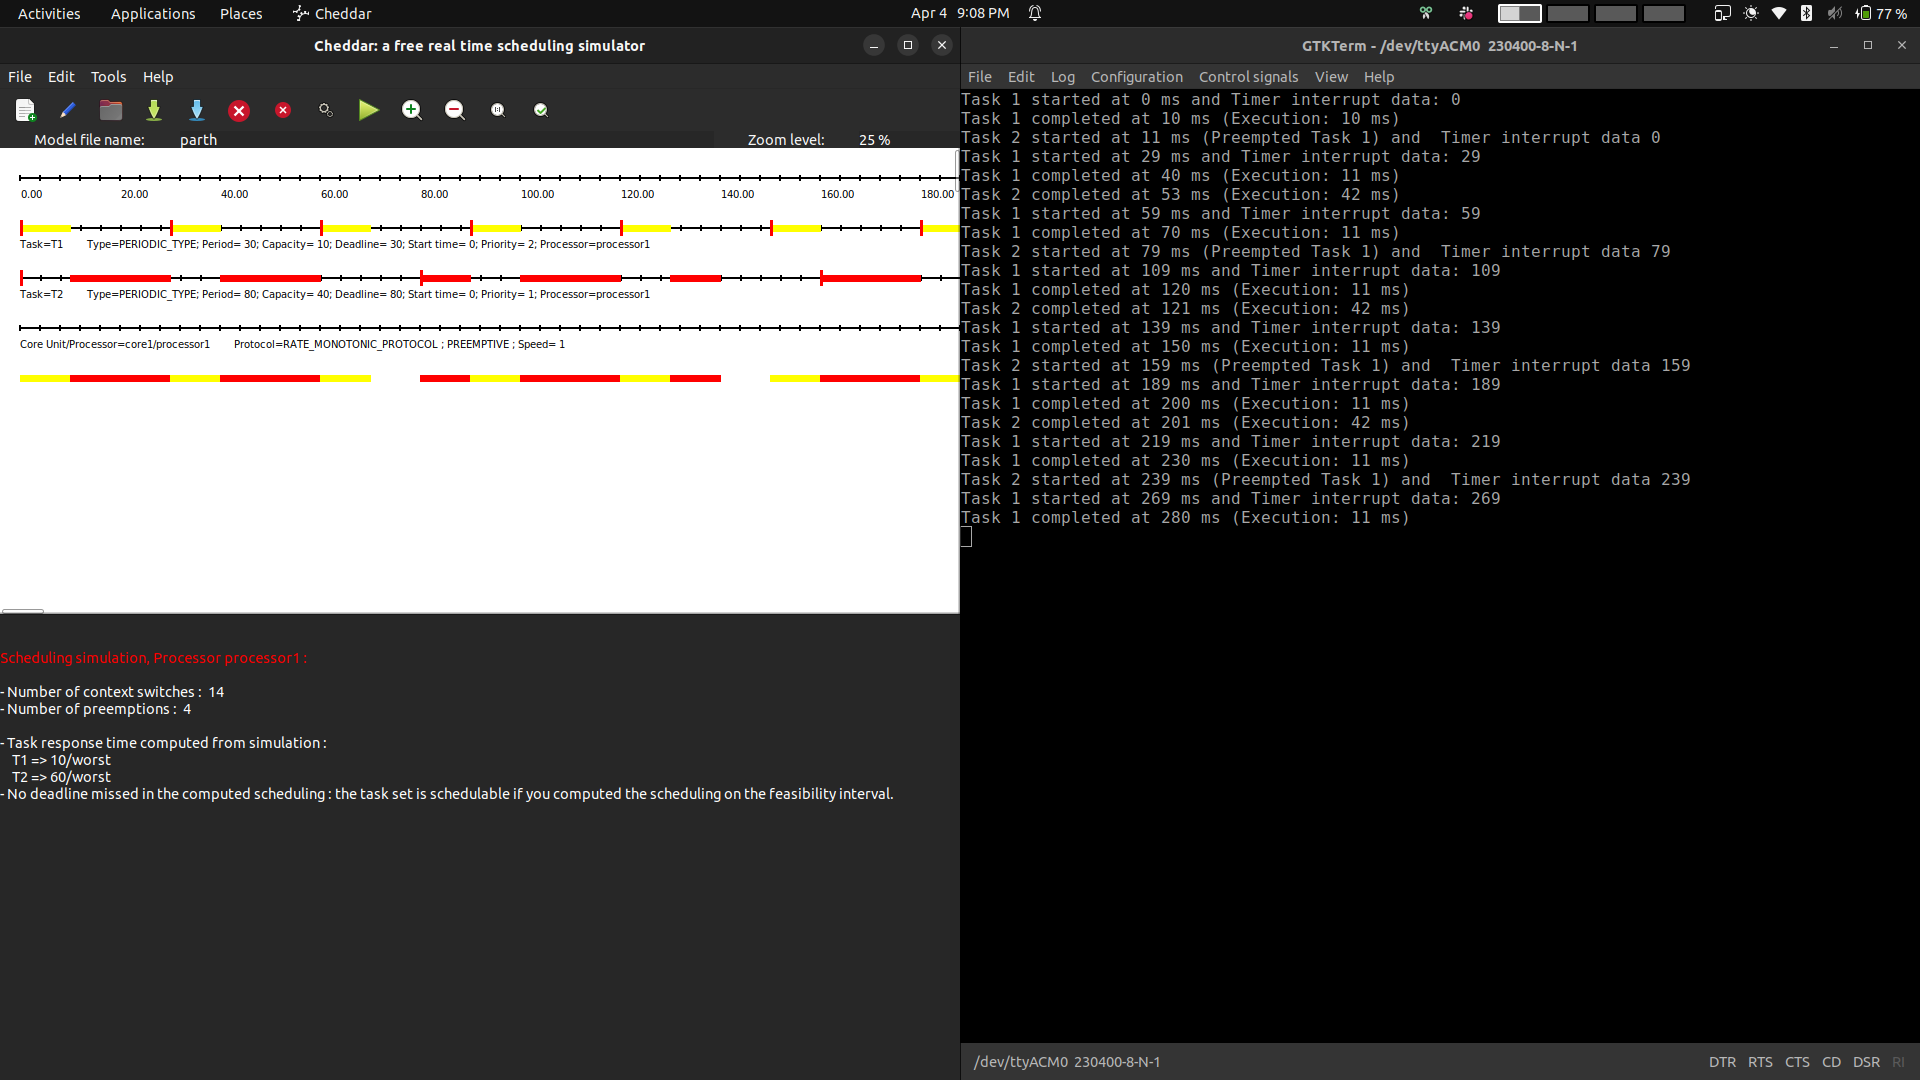
\includegraphics[scale=0.28]{figures/q3.png}
	\caption{Semaphore has been posted by this program}

\end{figure}
Output Analysis:
The provided output shows the execution timeline of Task 1 and Task 2 based on the timer interrupts and task notifications.
\begin{enumerate}
	\item  The output starts with Task 1 executing at 0 ms and completing at 10 ms, with an execution duration of 10 ms.
	\item Task 1 starts again at 29 ms (preempted by Task 1) and completes at 40 ms, with an execution duration of 11 ms.
	\item Task 2 starts at 53 ms (preempting Task 1) and completes at 95 ms, with an execution duration of 42 ms.
	\item The pattern continues, with Task 1 and Task 2 alternating their execution based on the timer interrupts.
	\item Task 1 executes for approximately 10-11 ms each time, while Task 2 executes for approximately 42 ms each time.
	\item  The timer interrupt data shows the tick count at which the task notification was received.
	\item The output demonstrates the successful synchronization and coordination of the tasks using timer interrupts and task notifications.
\end{enumerate}



The code showcases the usage of FreeRTOS tasks, timer interrupts, and task notifications to achieve a synchronized execution pattern between two tasks. The tasks perform computations for specified durations and are triggered by periodic timer interrupts. The output verifies the expected behavior, with Task 1 executing for shorter durations and Task 2 executing for longer durations, while being coordinated by the timer interrupts.




\end{qanda}
\pagebreak

\section{Referance}
\begin{enumerate}
	\item REAL-TIME EMBEDDED COMPONENTS AND SYSTEMS with LINUX and RTOS by Sam Siewert John Pratt
	\item Scheduling Algorithms for Multiprogramming in a Hard Real-Time Environment C. L. LIU AND JAMES W. LAYLAND
	\item https://bears.ece.ucsb.edu/class/ece253/lect7.pdf
\end{enumerate}


\vfill
\hrule
\vspace{0.5cm}

\pagebreak
\begin{appendices}
	\section{C Code for the Implementation}
	\subsection{Q1}
	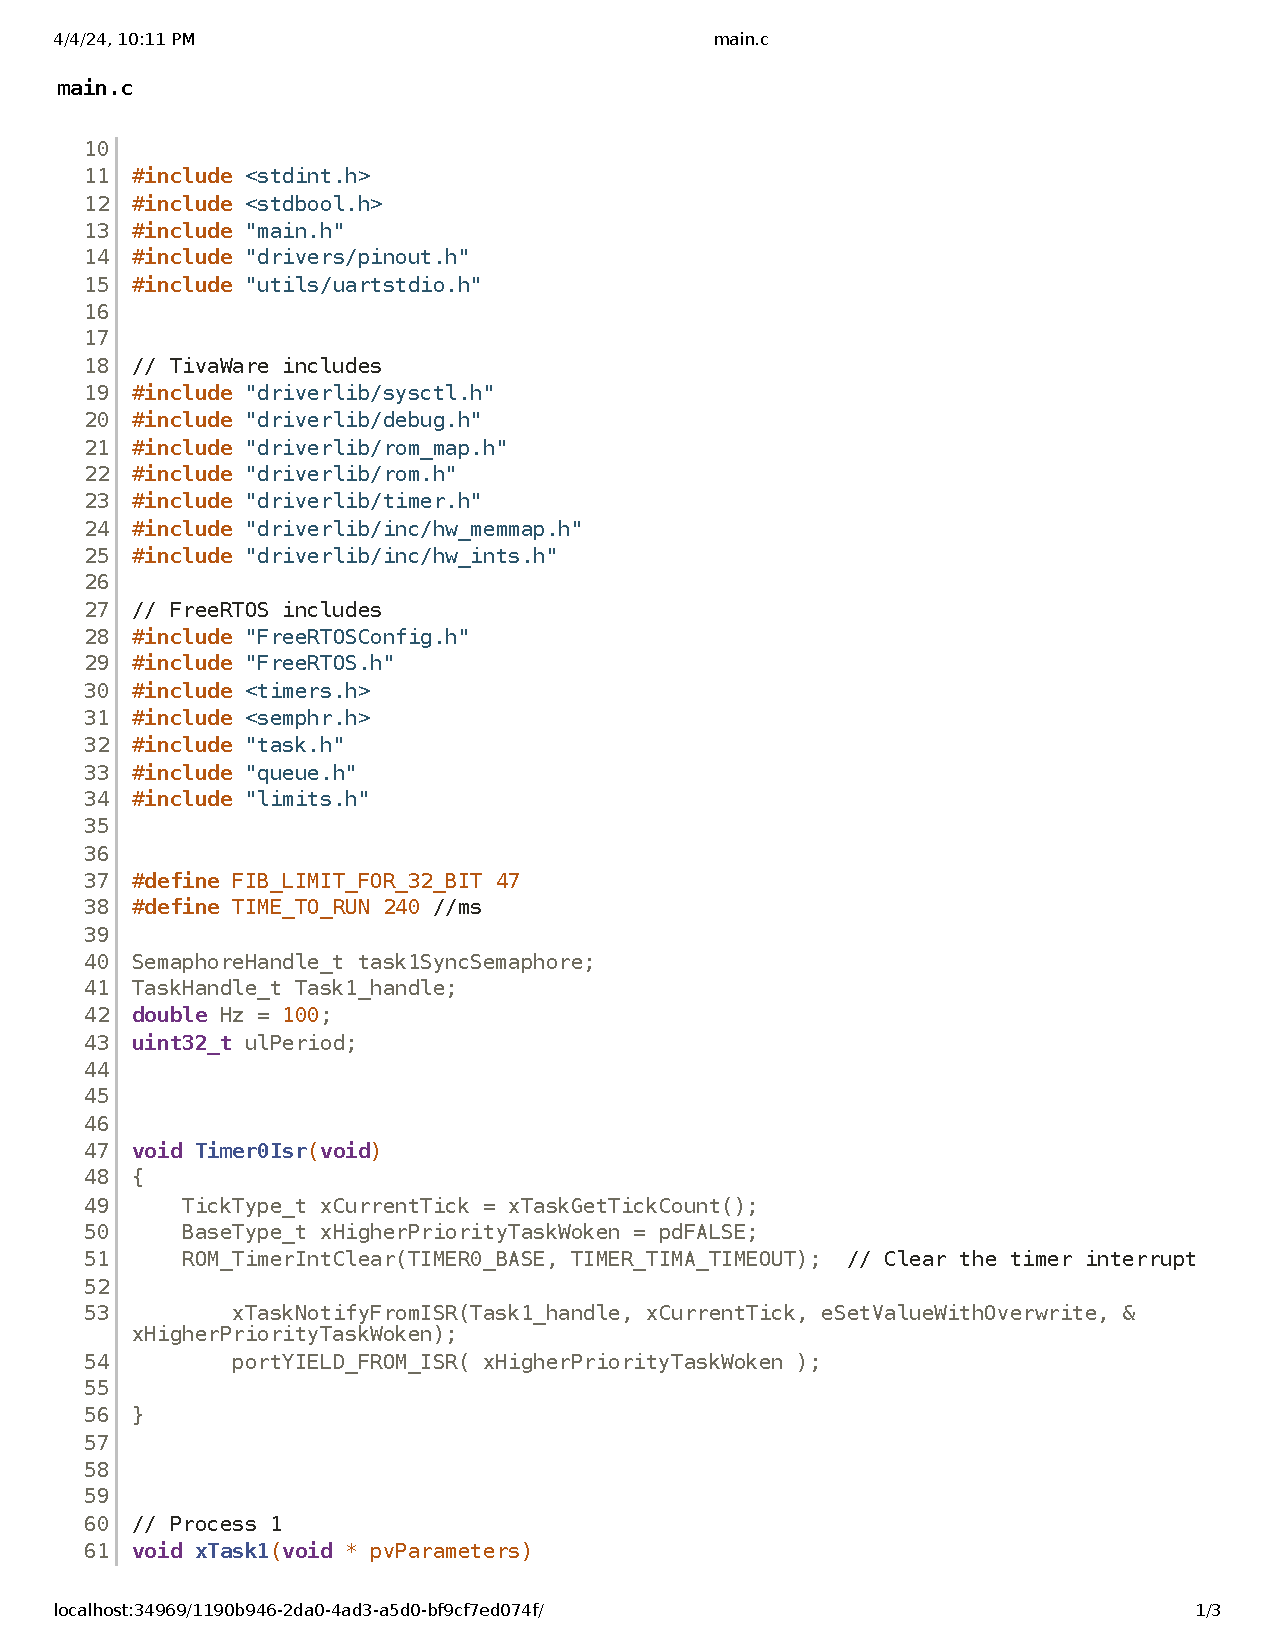
\includepdf[pages=-]{code/Q1.pdf}
	\pagebreak
	\subsection{Q2}
	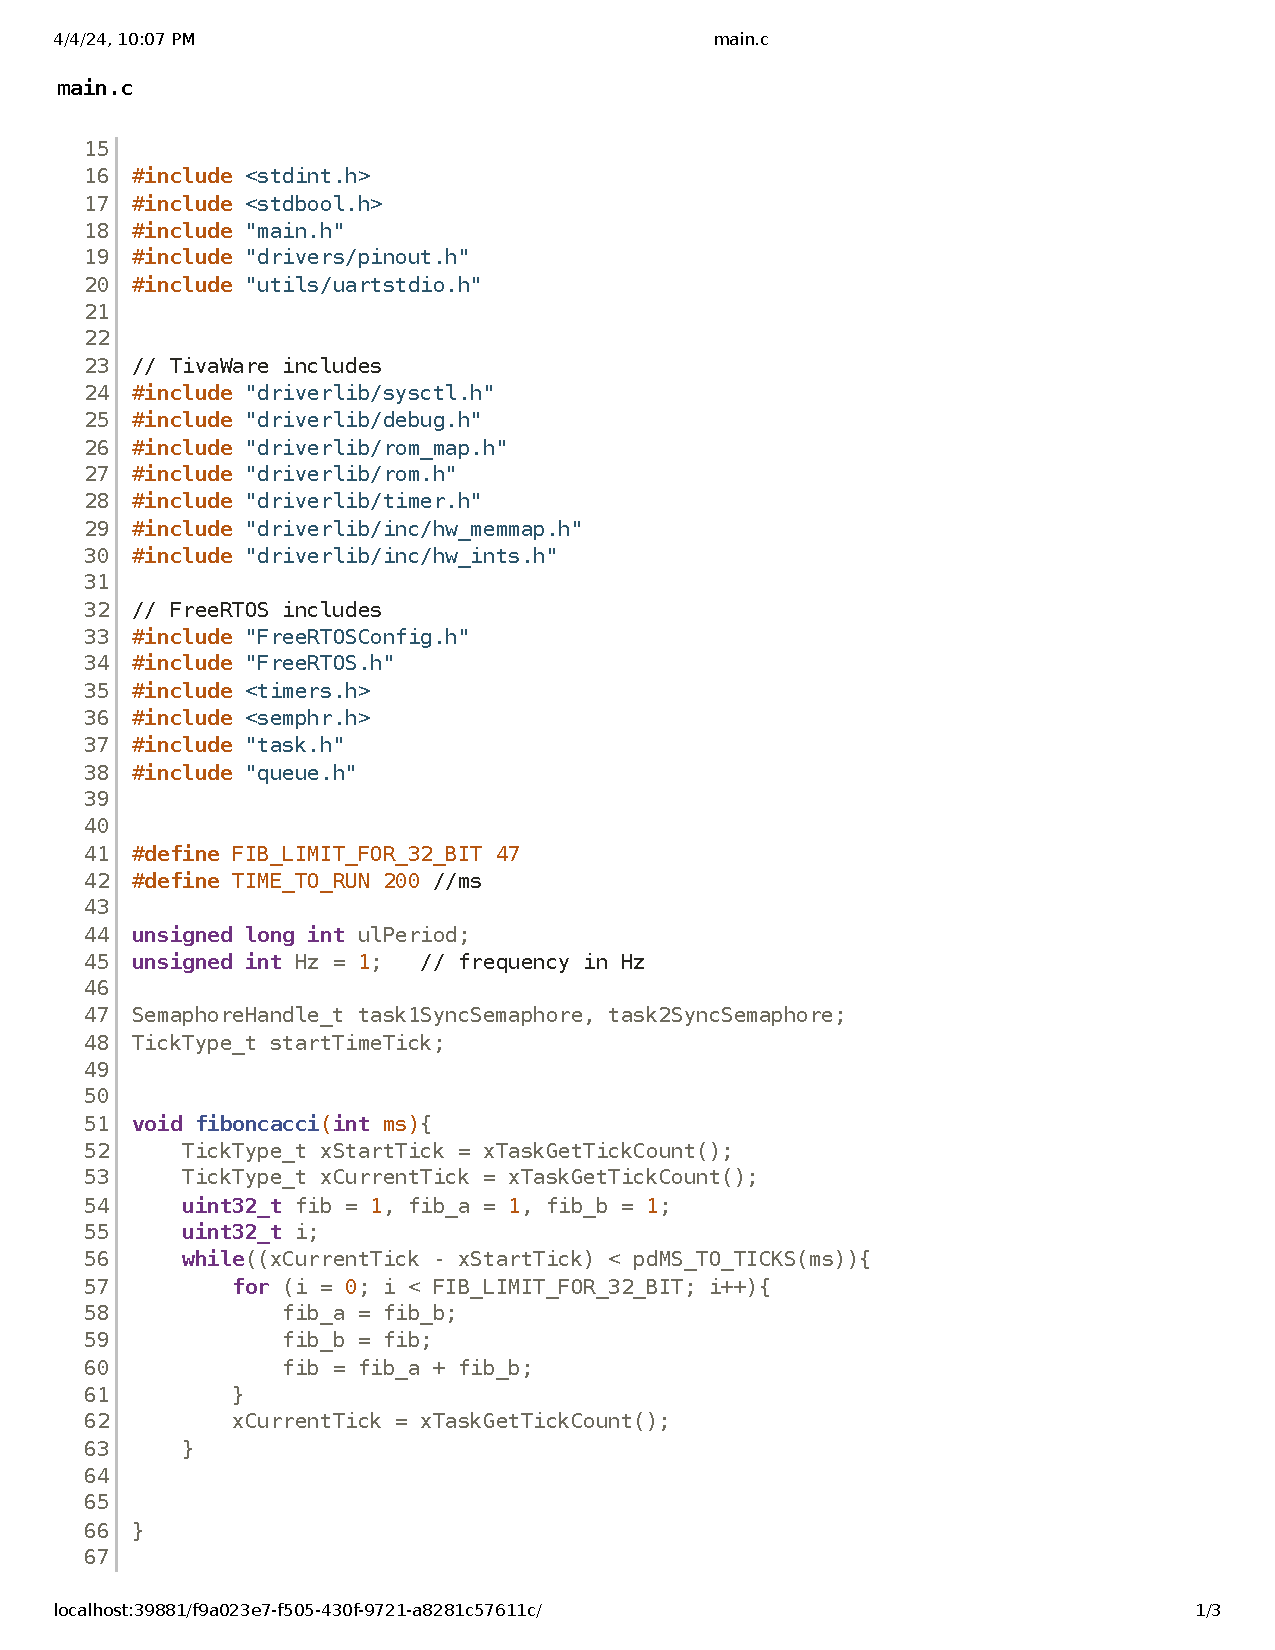
\includepdf[pages=-]{code/Q2.pdf}
	\pagebreak
	\subsection{Q3}
	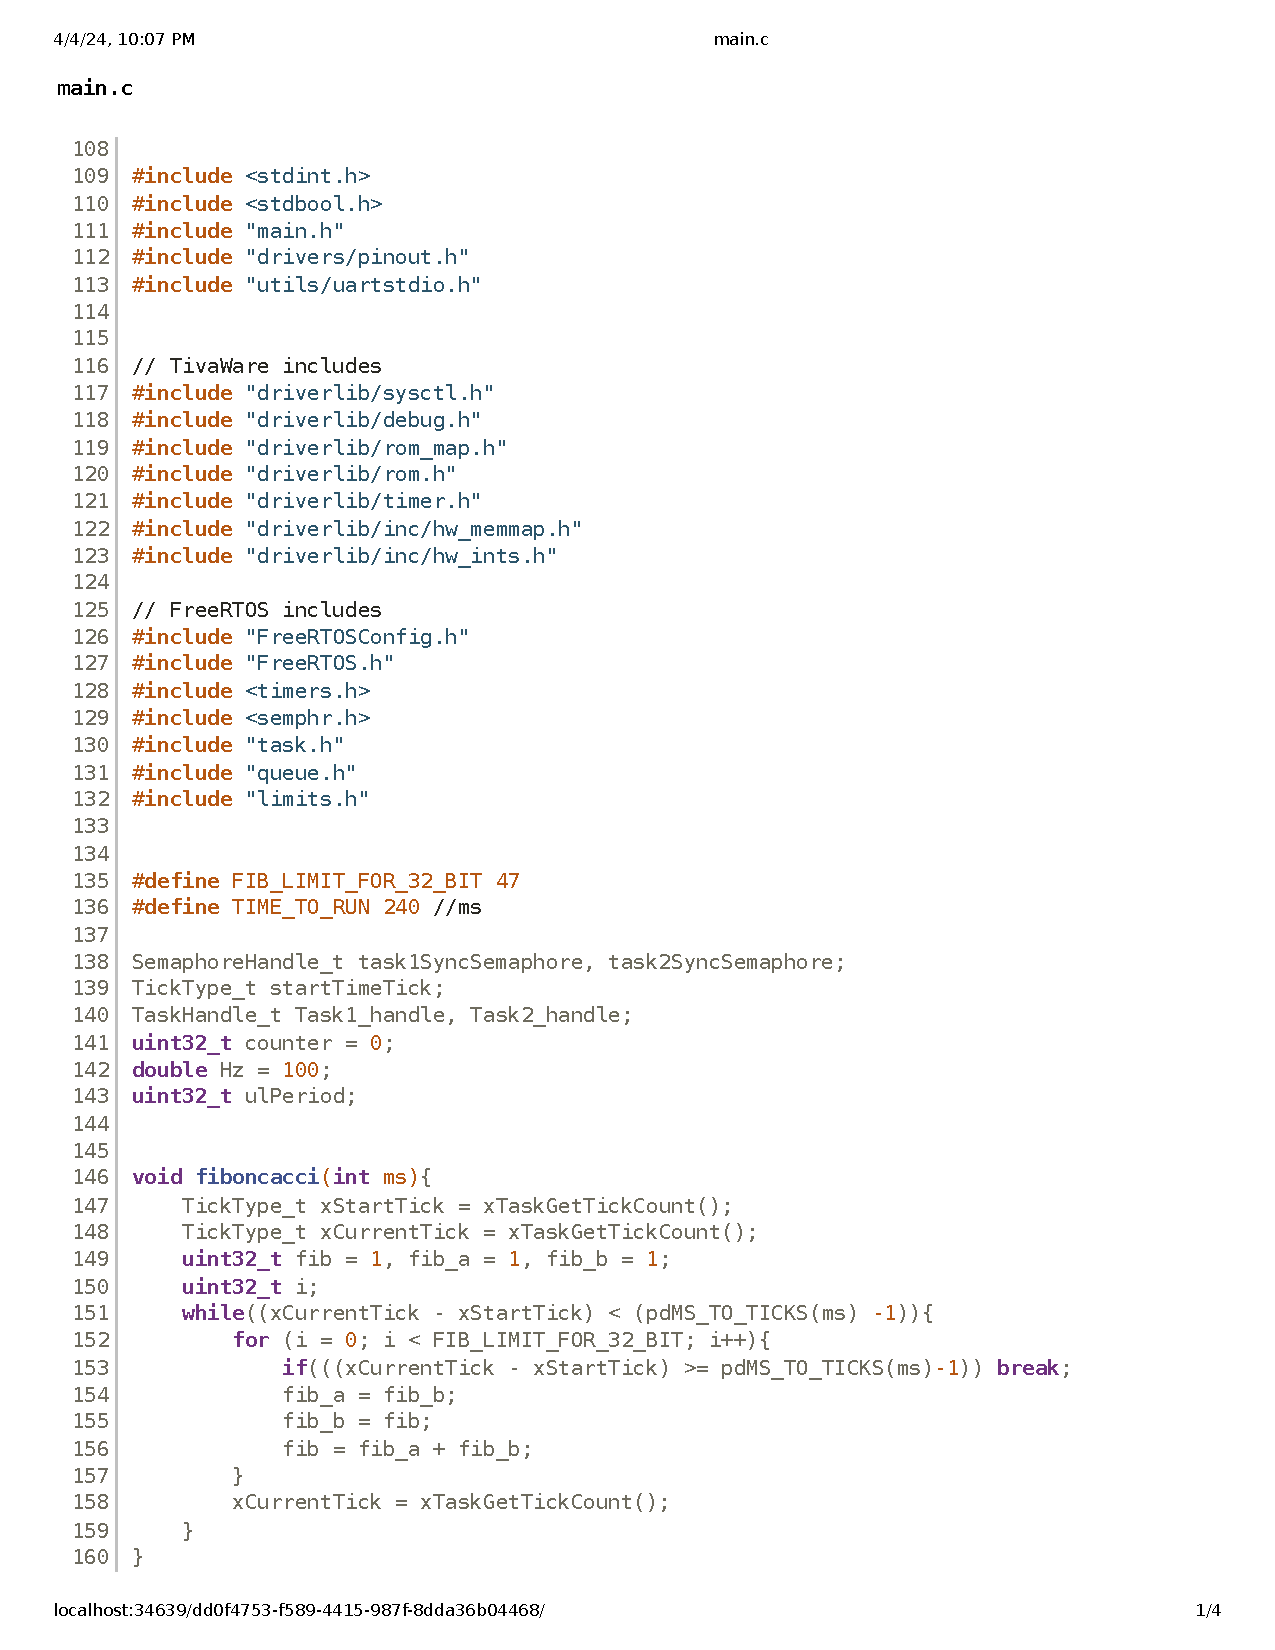
\includepdf[pages=-]{code/Q3.pdf}
	\pagebreak

\end{appendices}


\vspace{1cm}
\hrule
\vspace{0.5cm}


%---------------------------------------------------------------------------
\end{document}
-
